\subsection{The Model}
	The following model concerns the most characterizing features of the system. We avoided to burden the model with trivial and non-significant details.
	
	\subsubsection*{Data Types}
		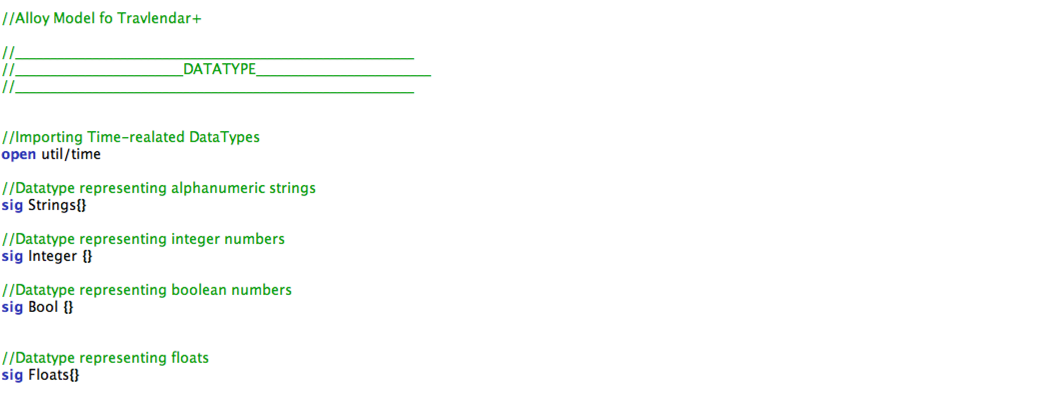
\includegraphics[width = \textwidth]{alloy/code/dataType}

	\subsubsection*{Signatures}
		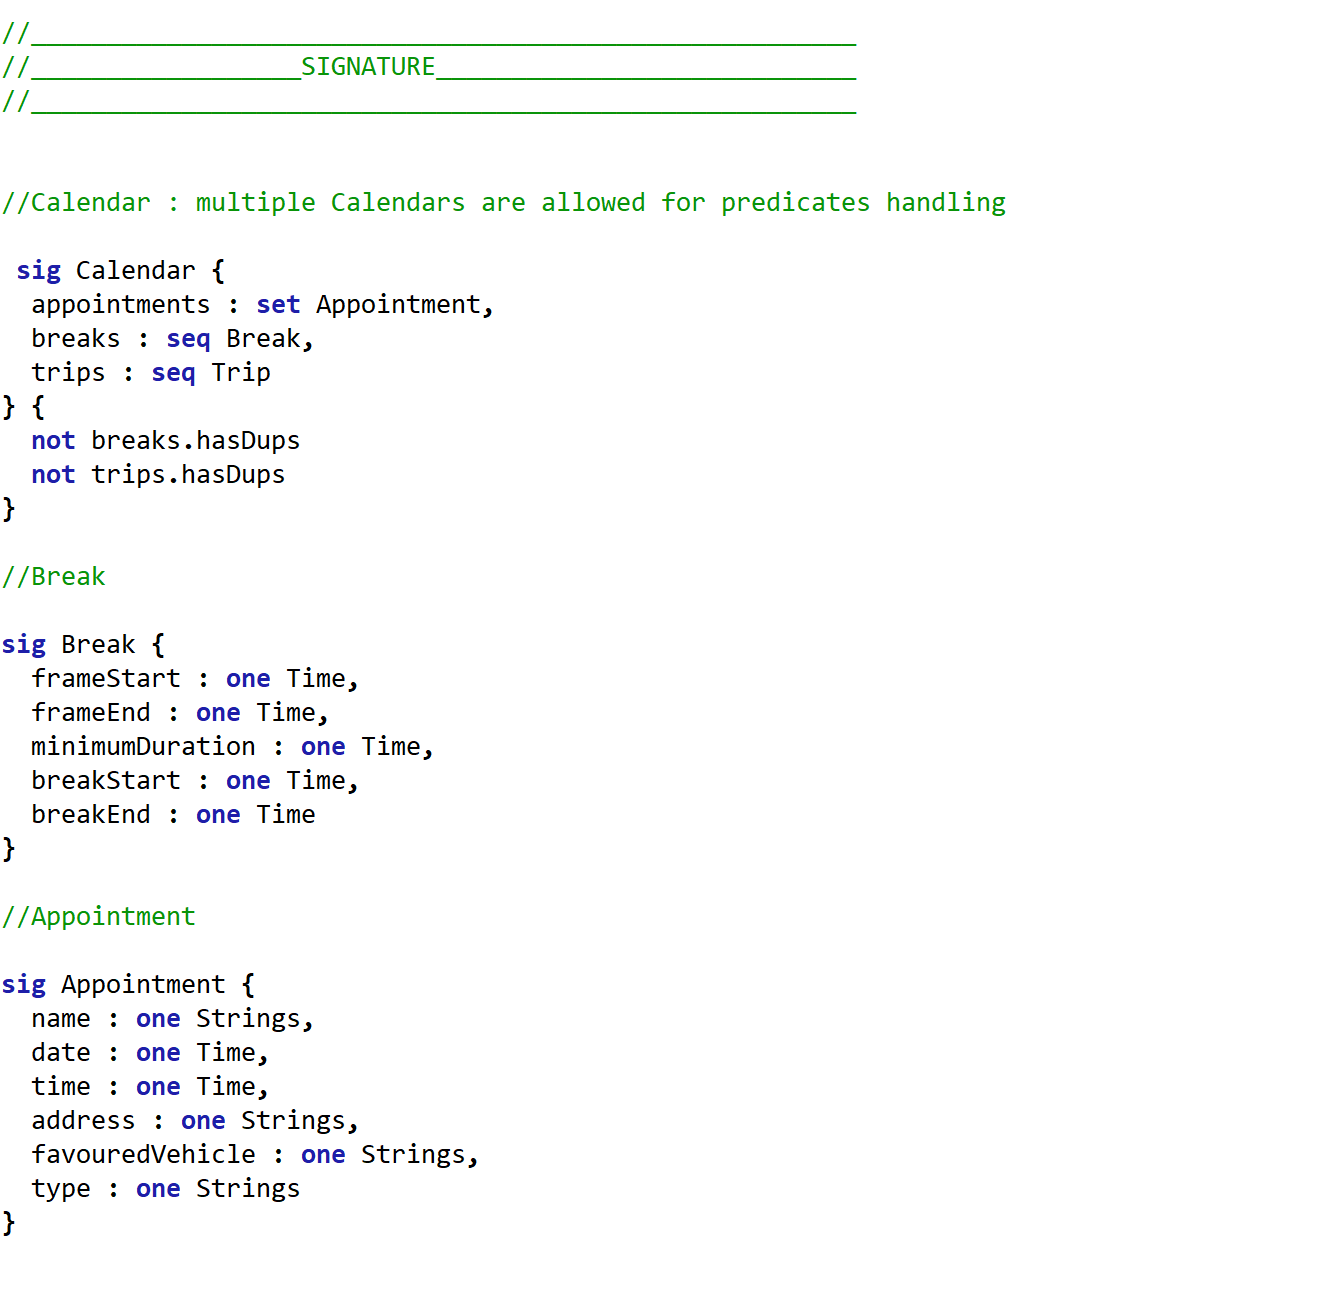
\includegraphics[width = \textwidth]{alloy/code/signature1}
		\vfill
		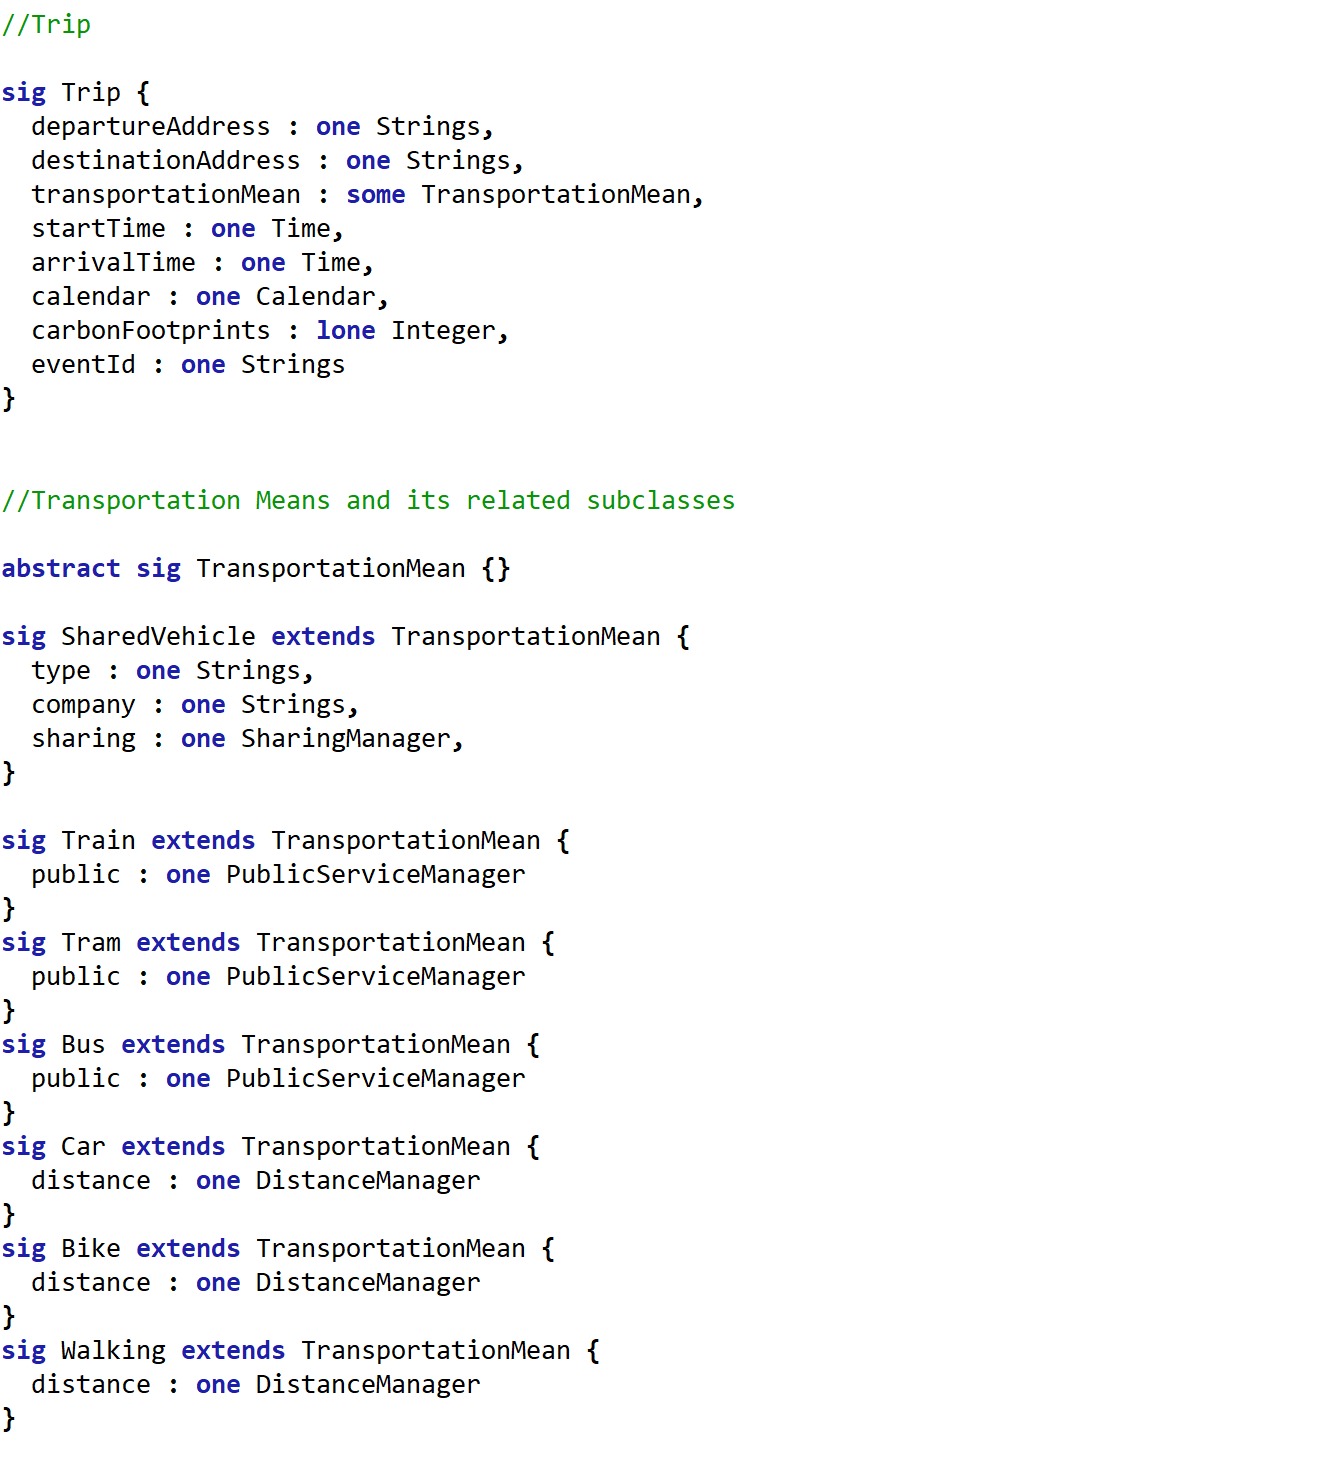
\includegraphics[width = \textwidth]{alloy/code/signature2}
	
	\subsubsection*{Facts}
		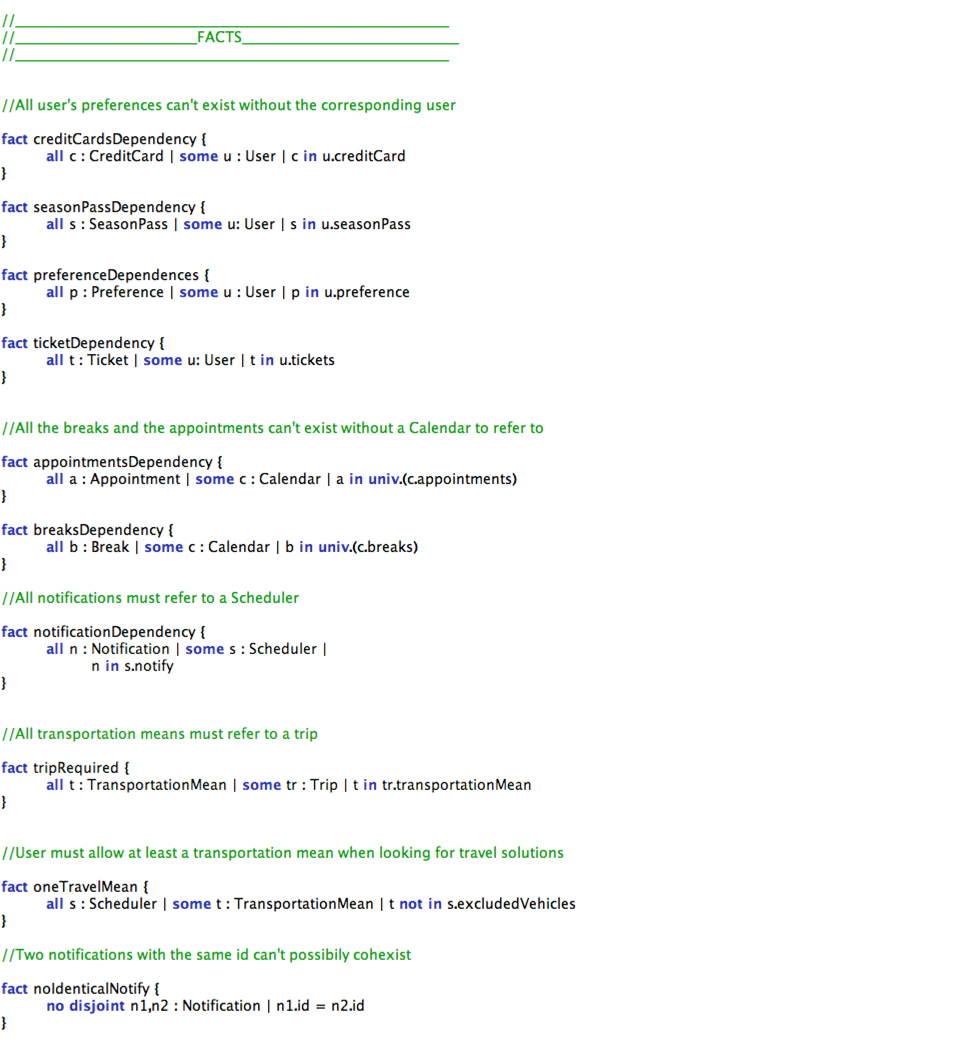
\includegraphics[width = \textwidth]{alloy/code/fact1}
		\vfill
		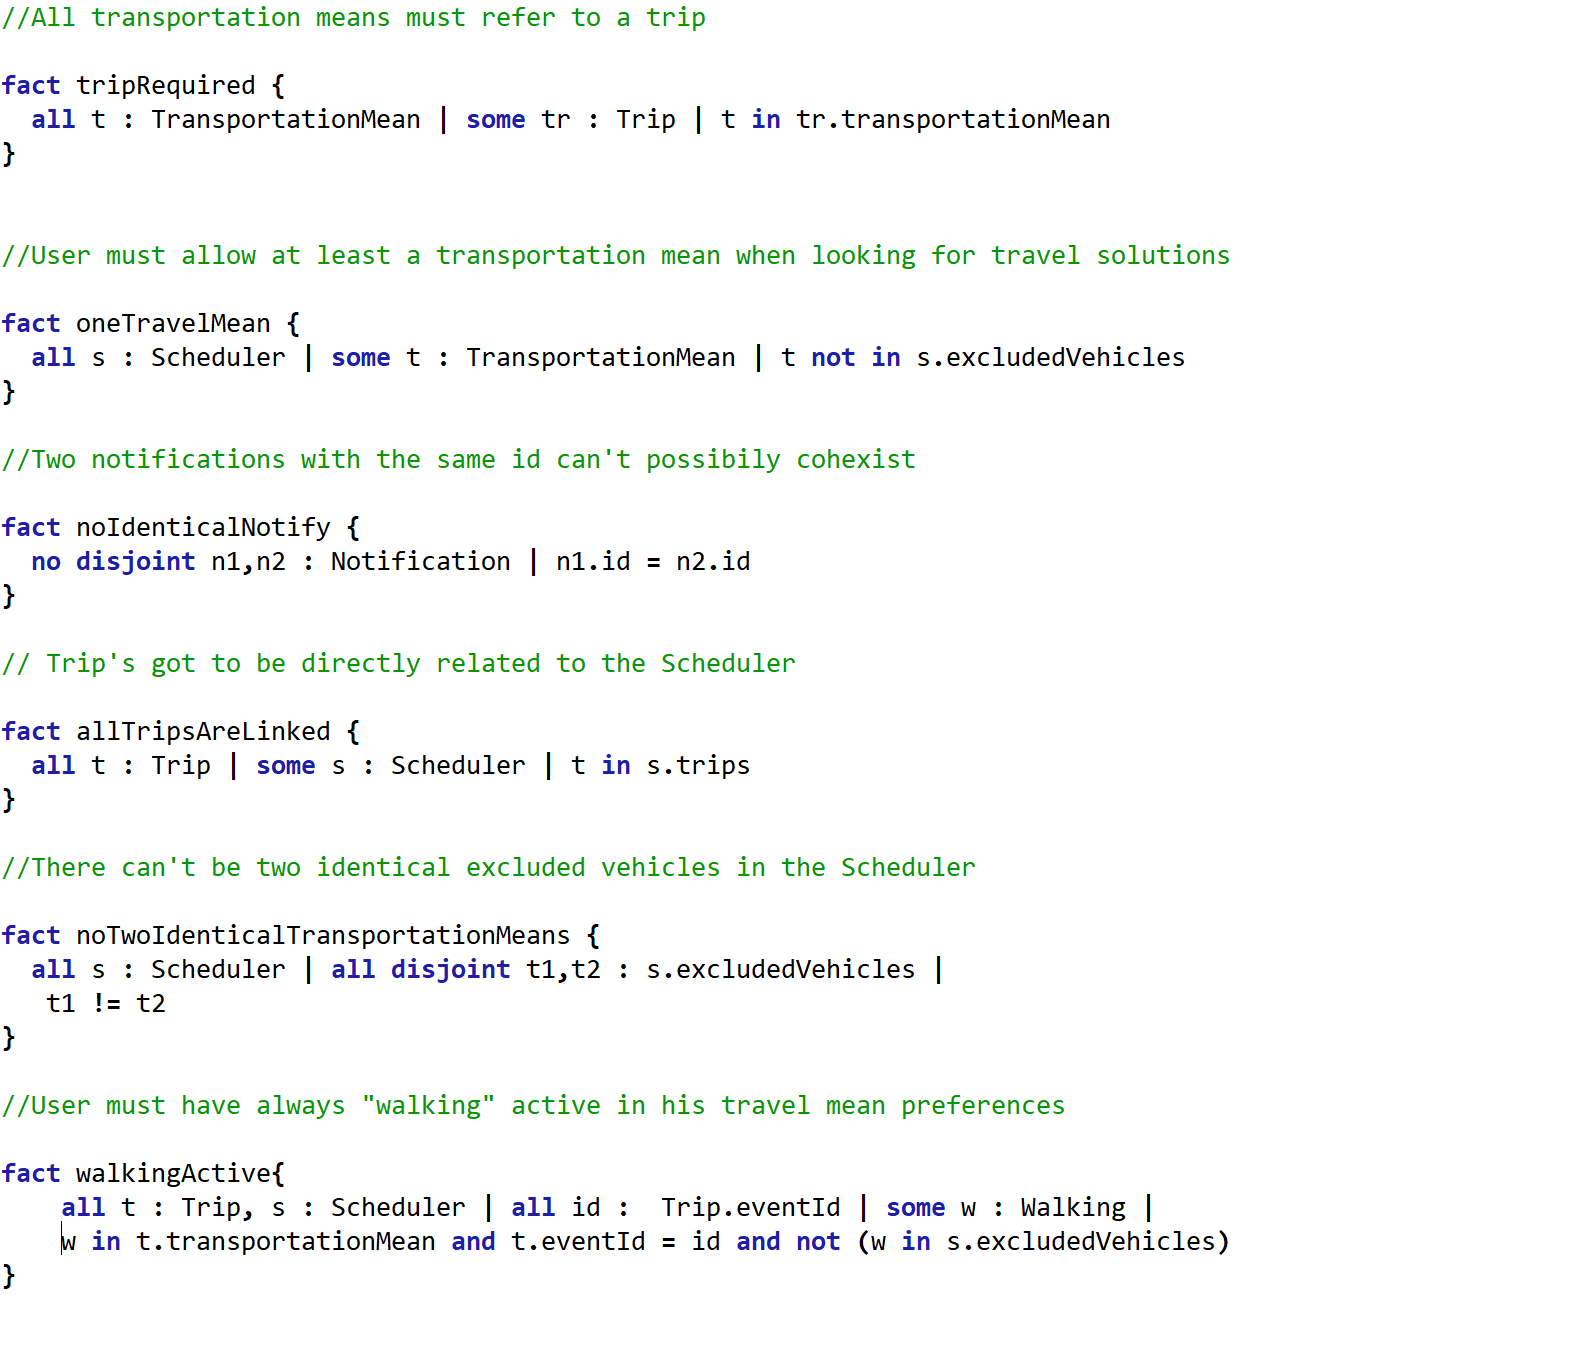
\includegraphics[width = \textwidth]{alloy/code/fact2}
	
	\subsubsection*{Predicates}
		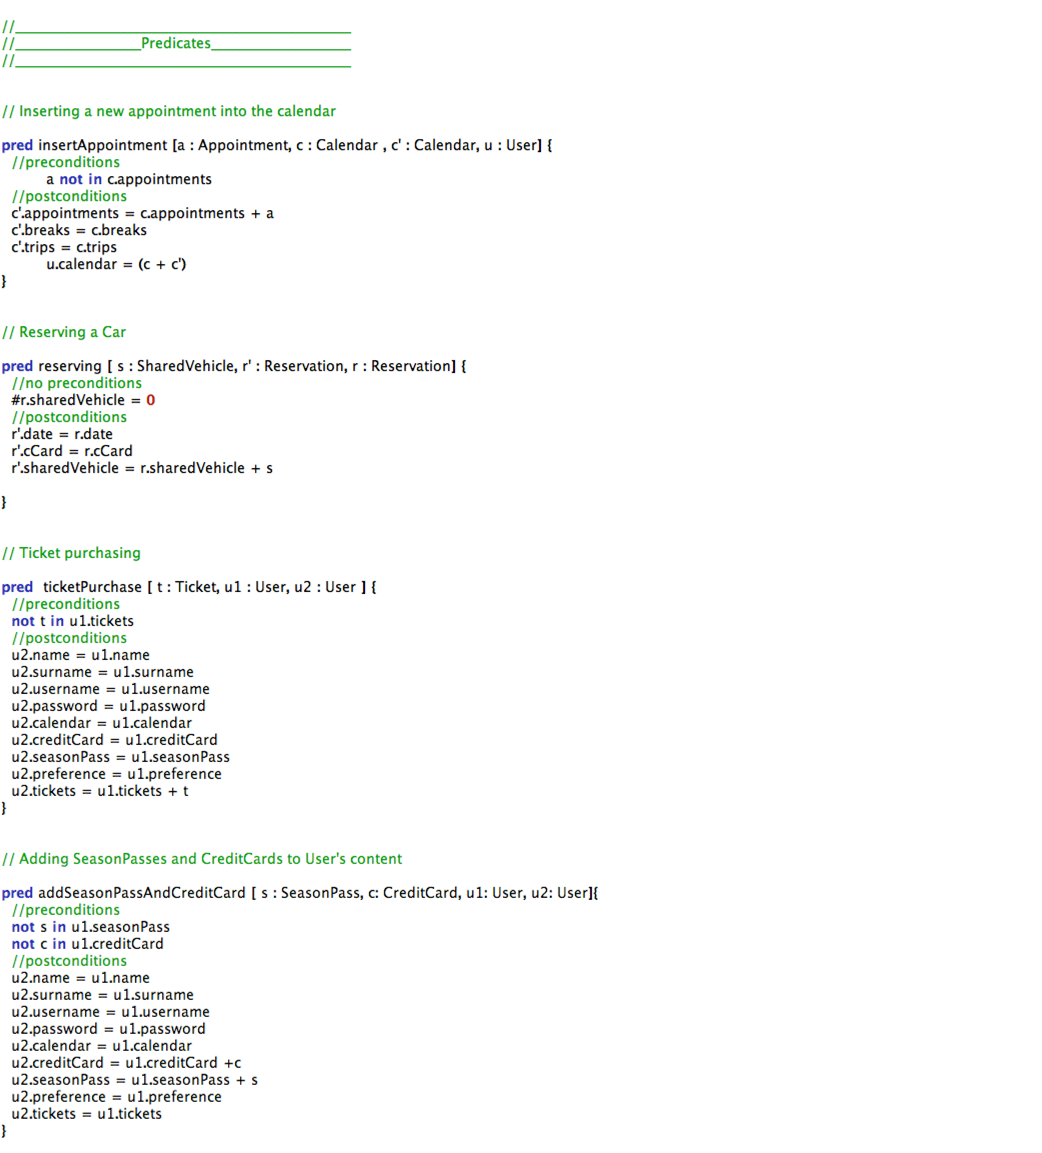
\includegraphics[width = \textwidth]{alloy/code/predicate}
		\bigskip
		
\subsection{Results}
	\begin{figure}[H]
		\centering
		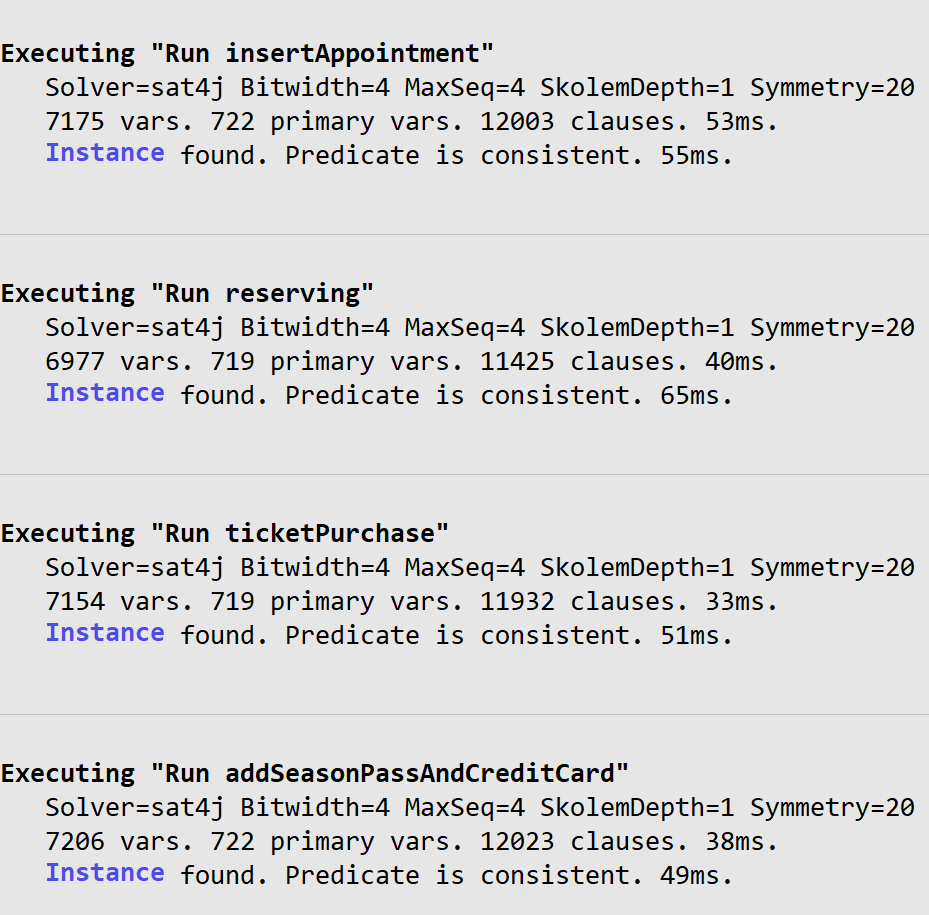
\includegraphics[width = 0.7\linewidth]{alloy/generatedWorld/Results}
		\caption{Result of the model analysis.}		
		\label{fig:alloyResult}
	\end{figure}
	\bigskip
	
	
	
	

\begin{landscape}
	\subsection{Generated World}
	
		\subsubsection{World Generated}
			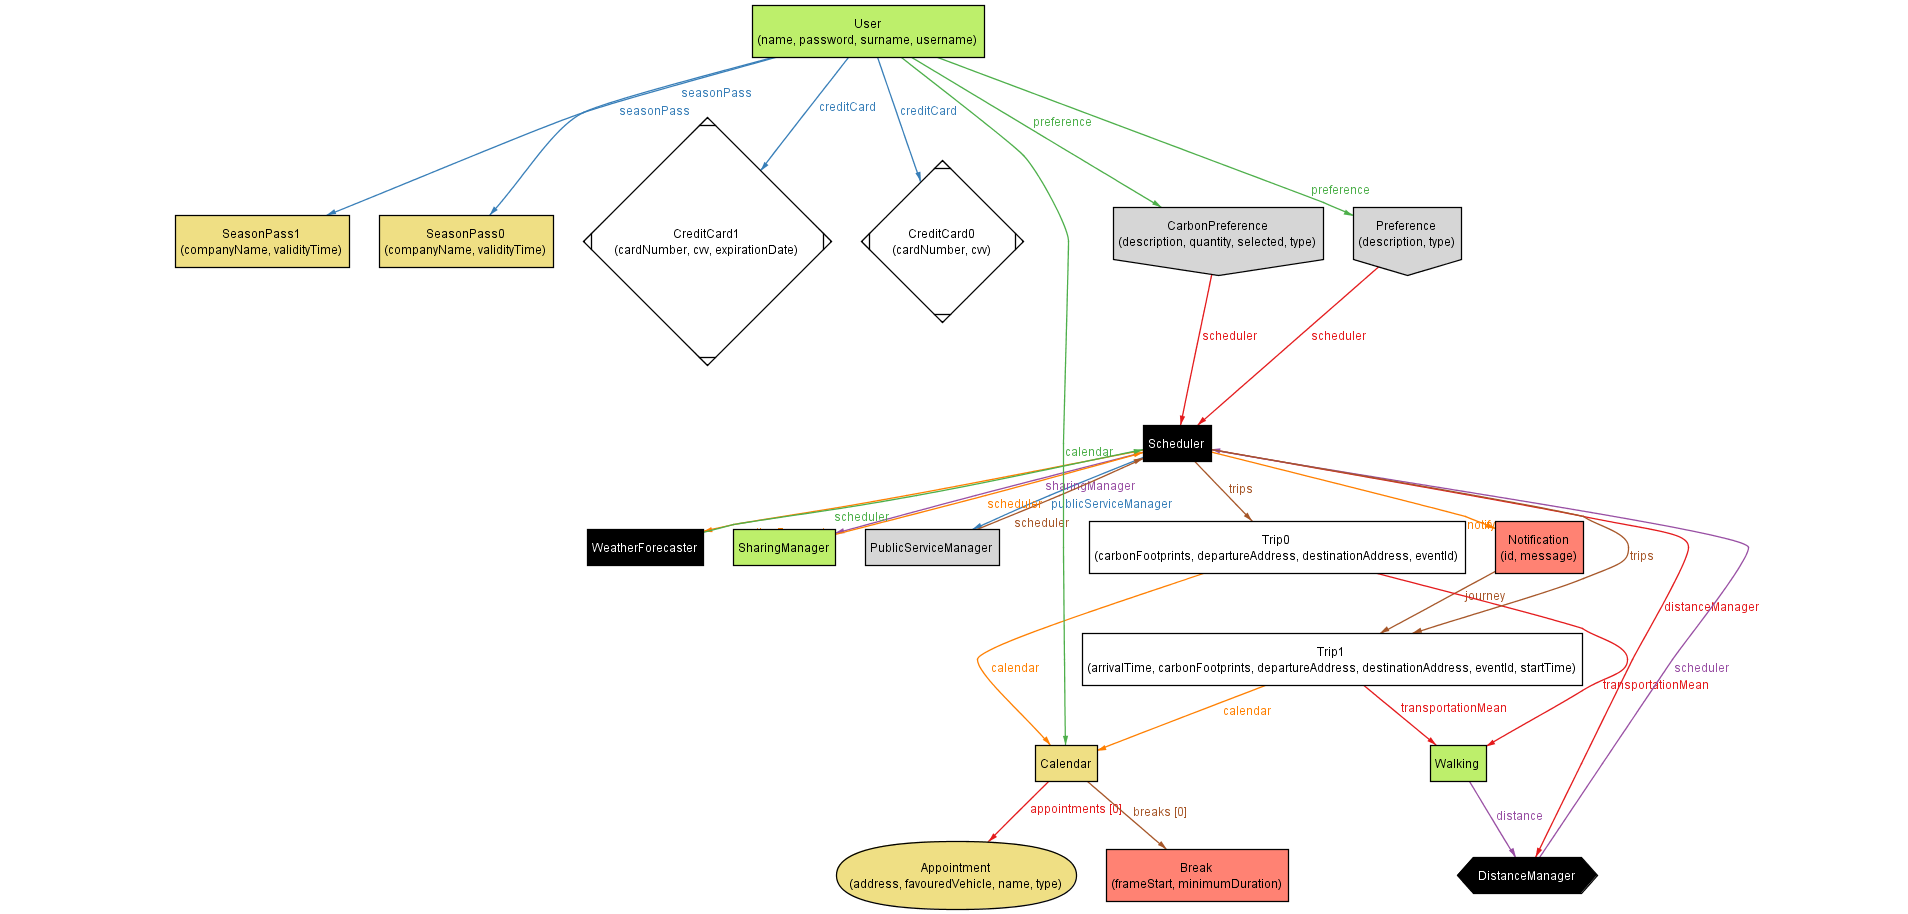
\includegraphics[height= 0.9\textheight , center]{alloy/generatedWorld/WorldGenerated}
	
		\subsubsection{Ticket Purchase}
			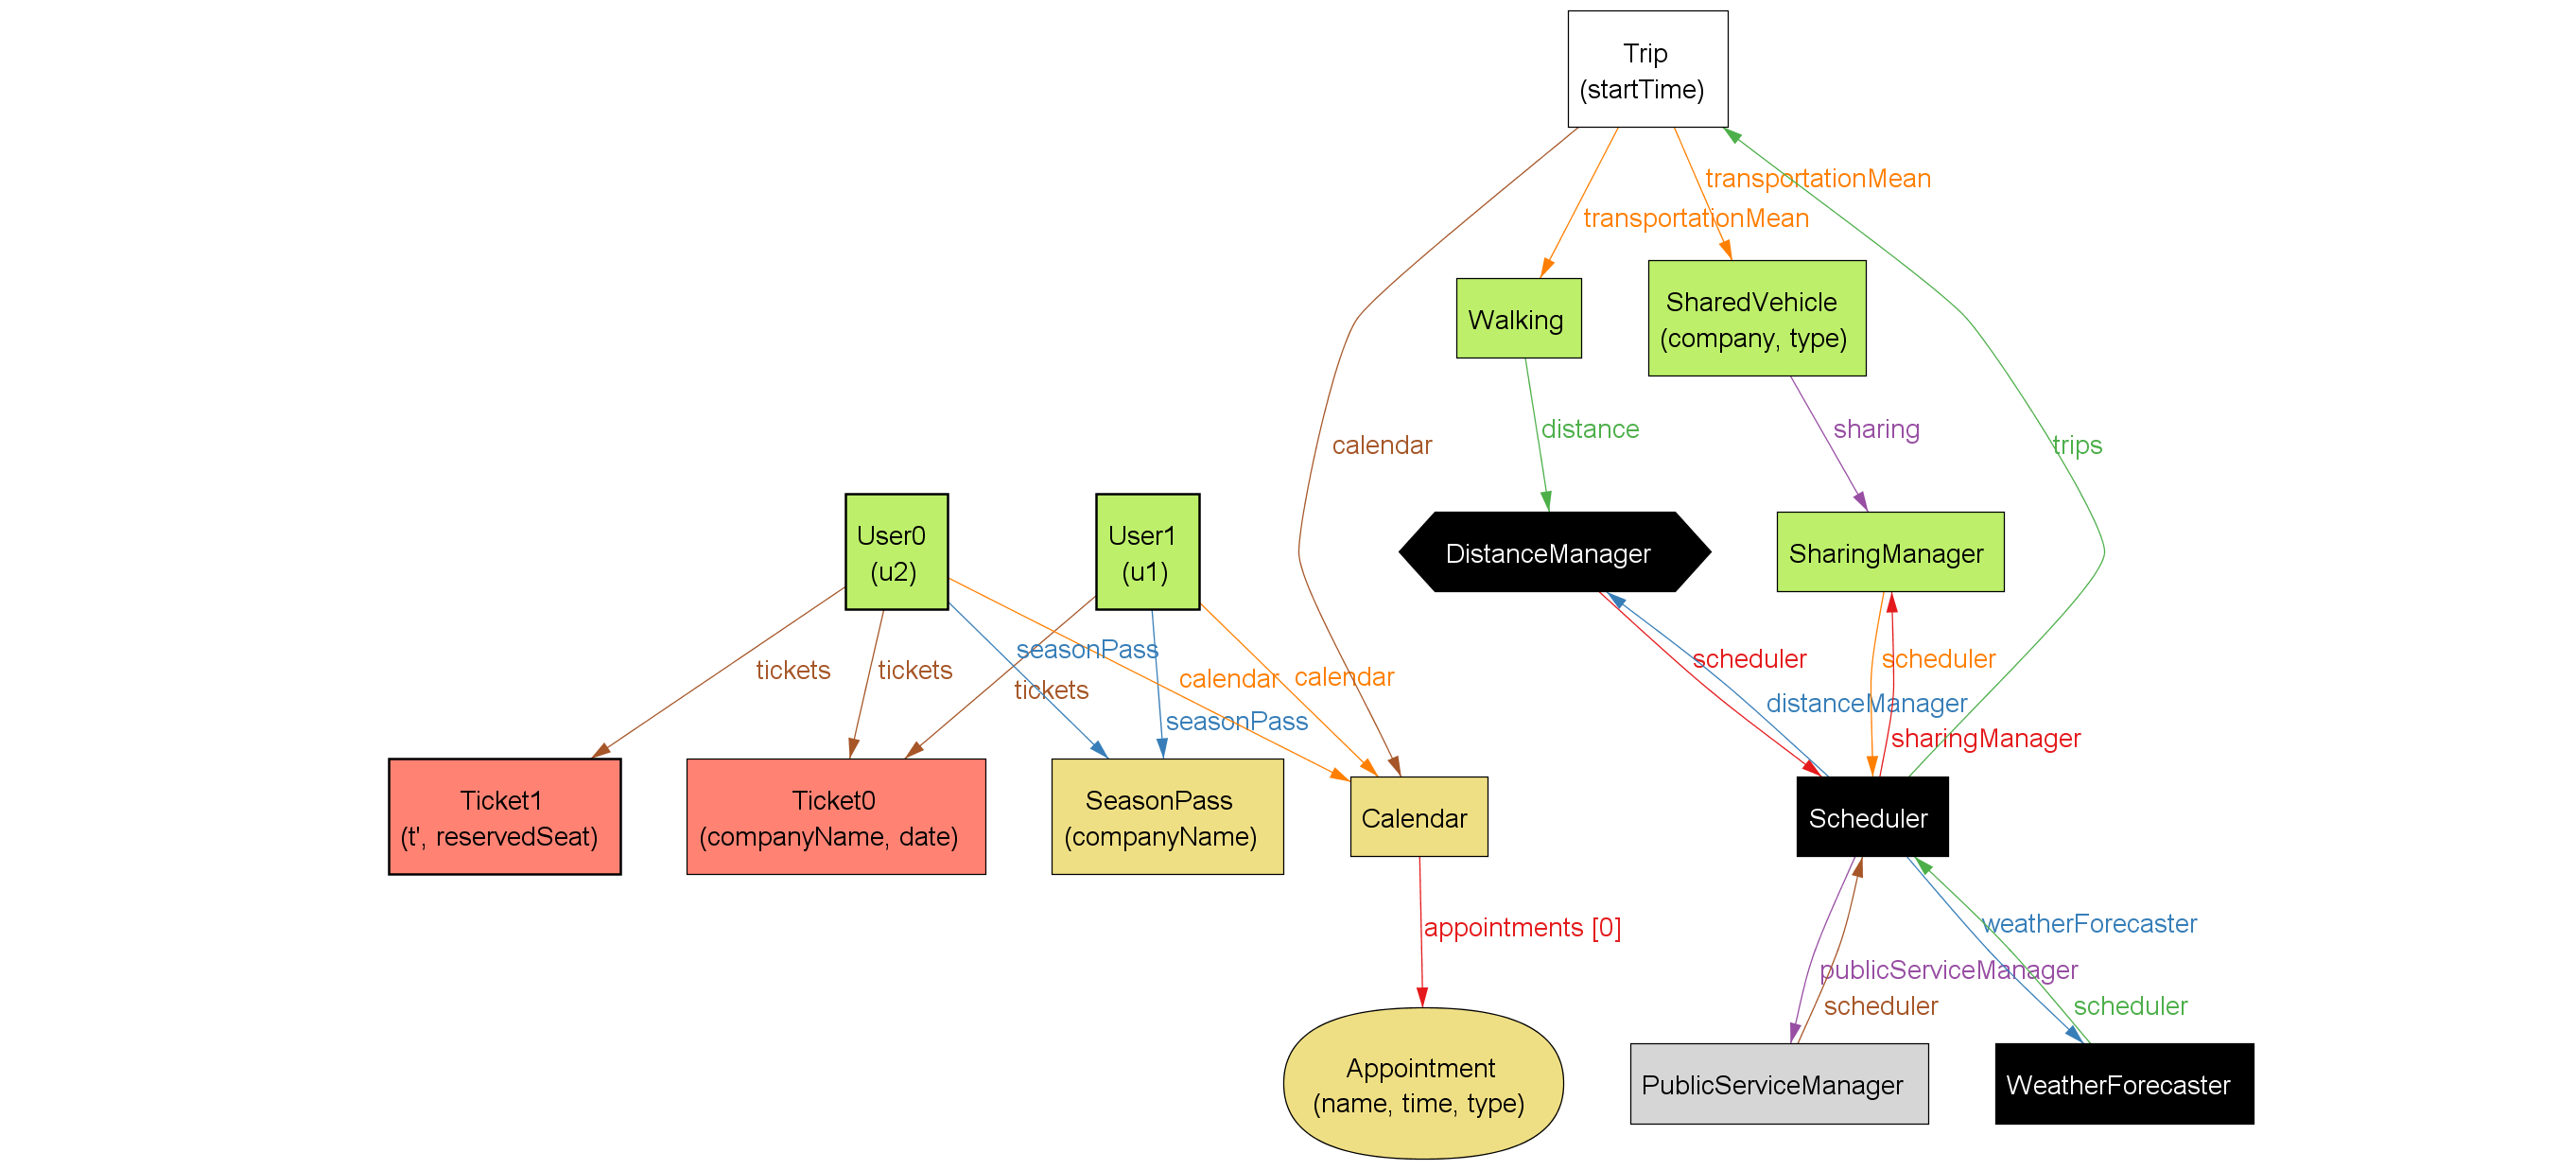
\includegraphics[height= 0.9\textheight, width= 35cm, center]{alloy/generatedWorld/ticketPurchase}
	
		\subsubsection{Renting}
			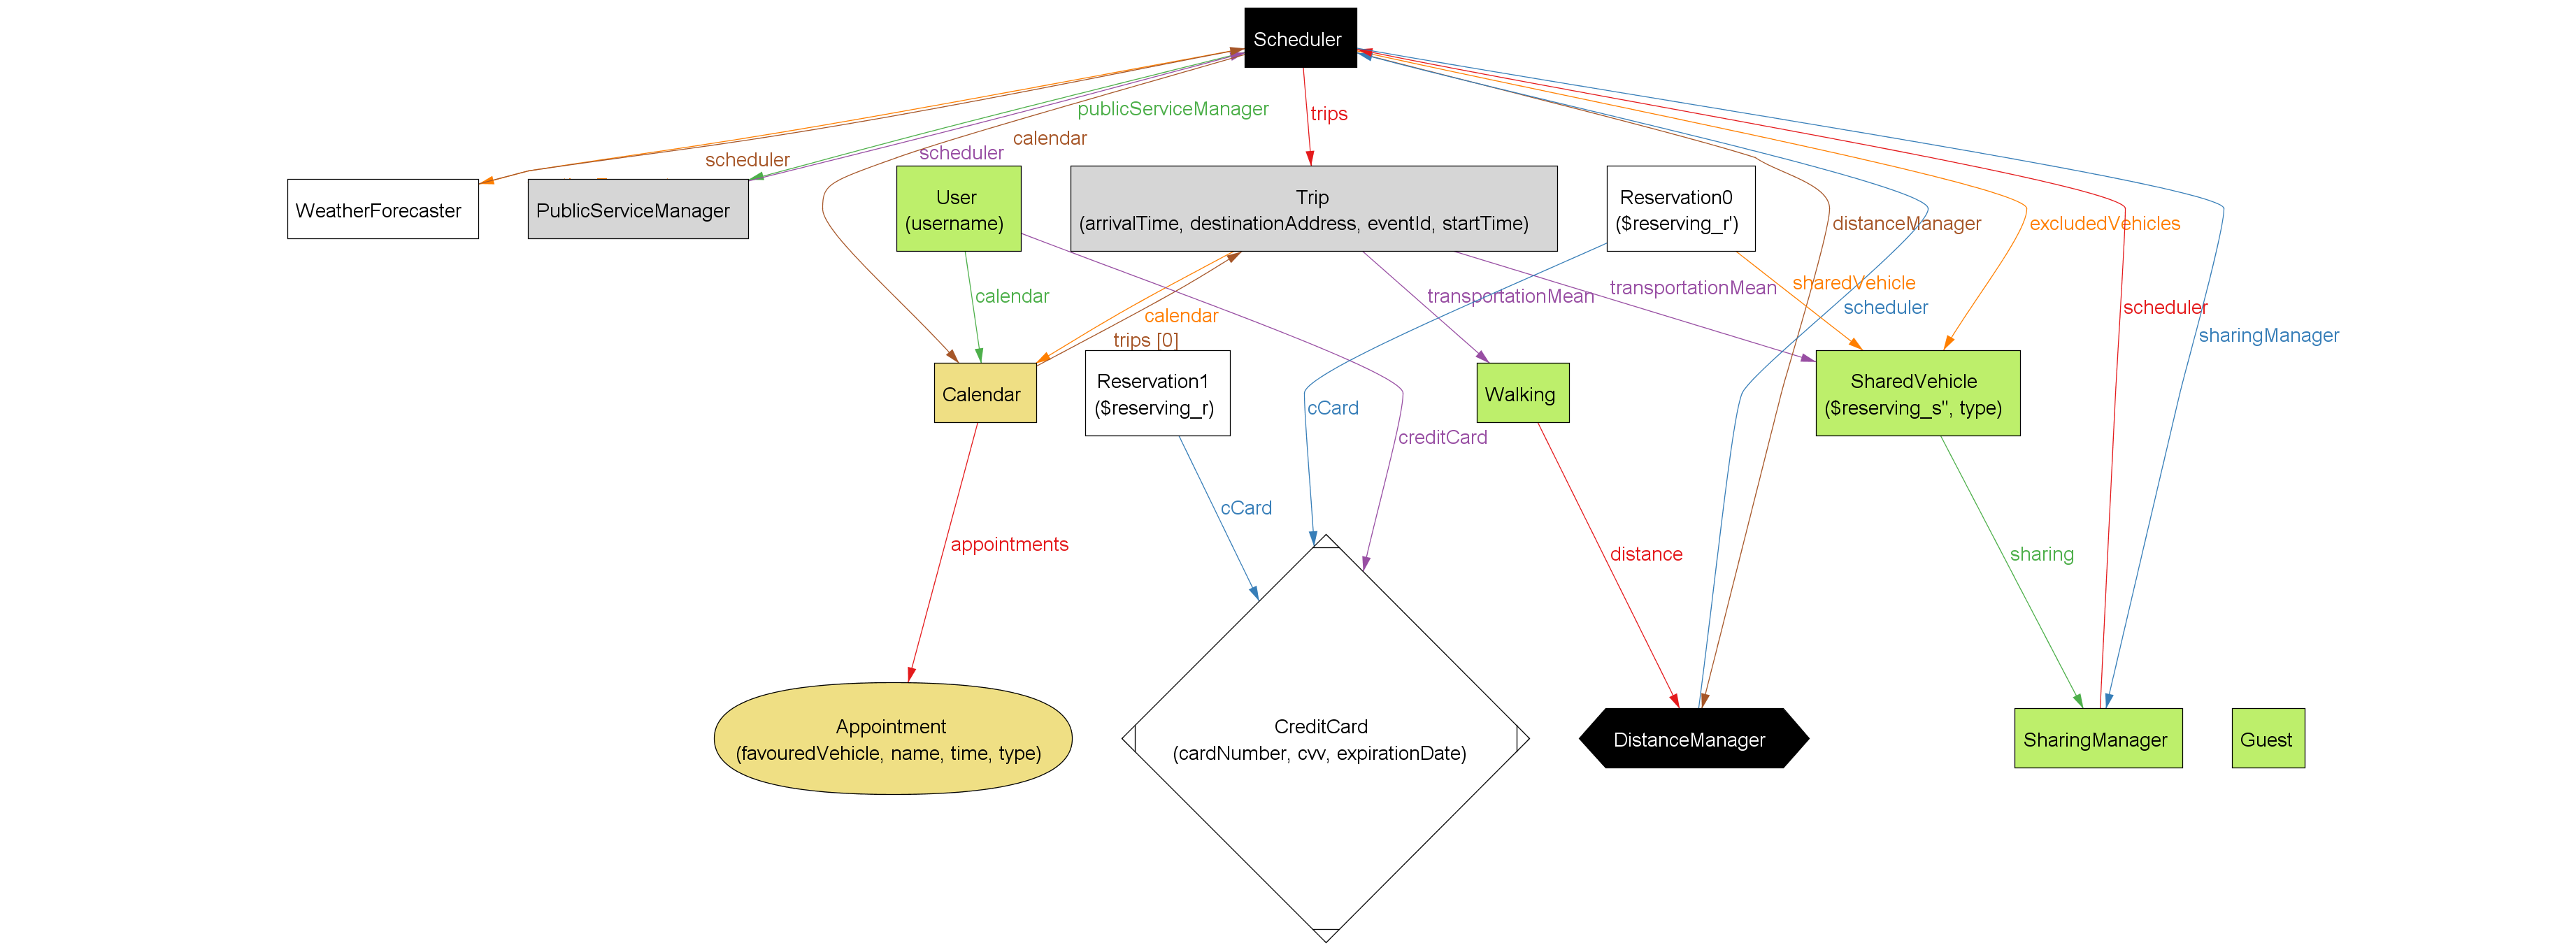
\includegraphics[height = 0.9\textheight, width= 35cm, center]{alloy/generatedWorld/reserving}
		
		\subsubsection{Insert Appointment}
			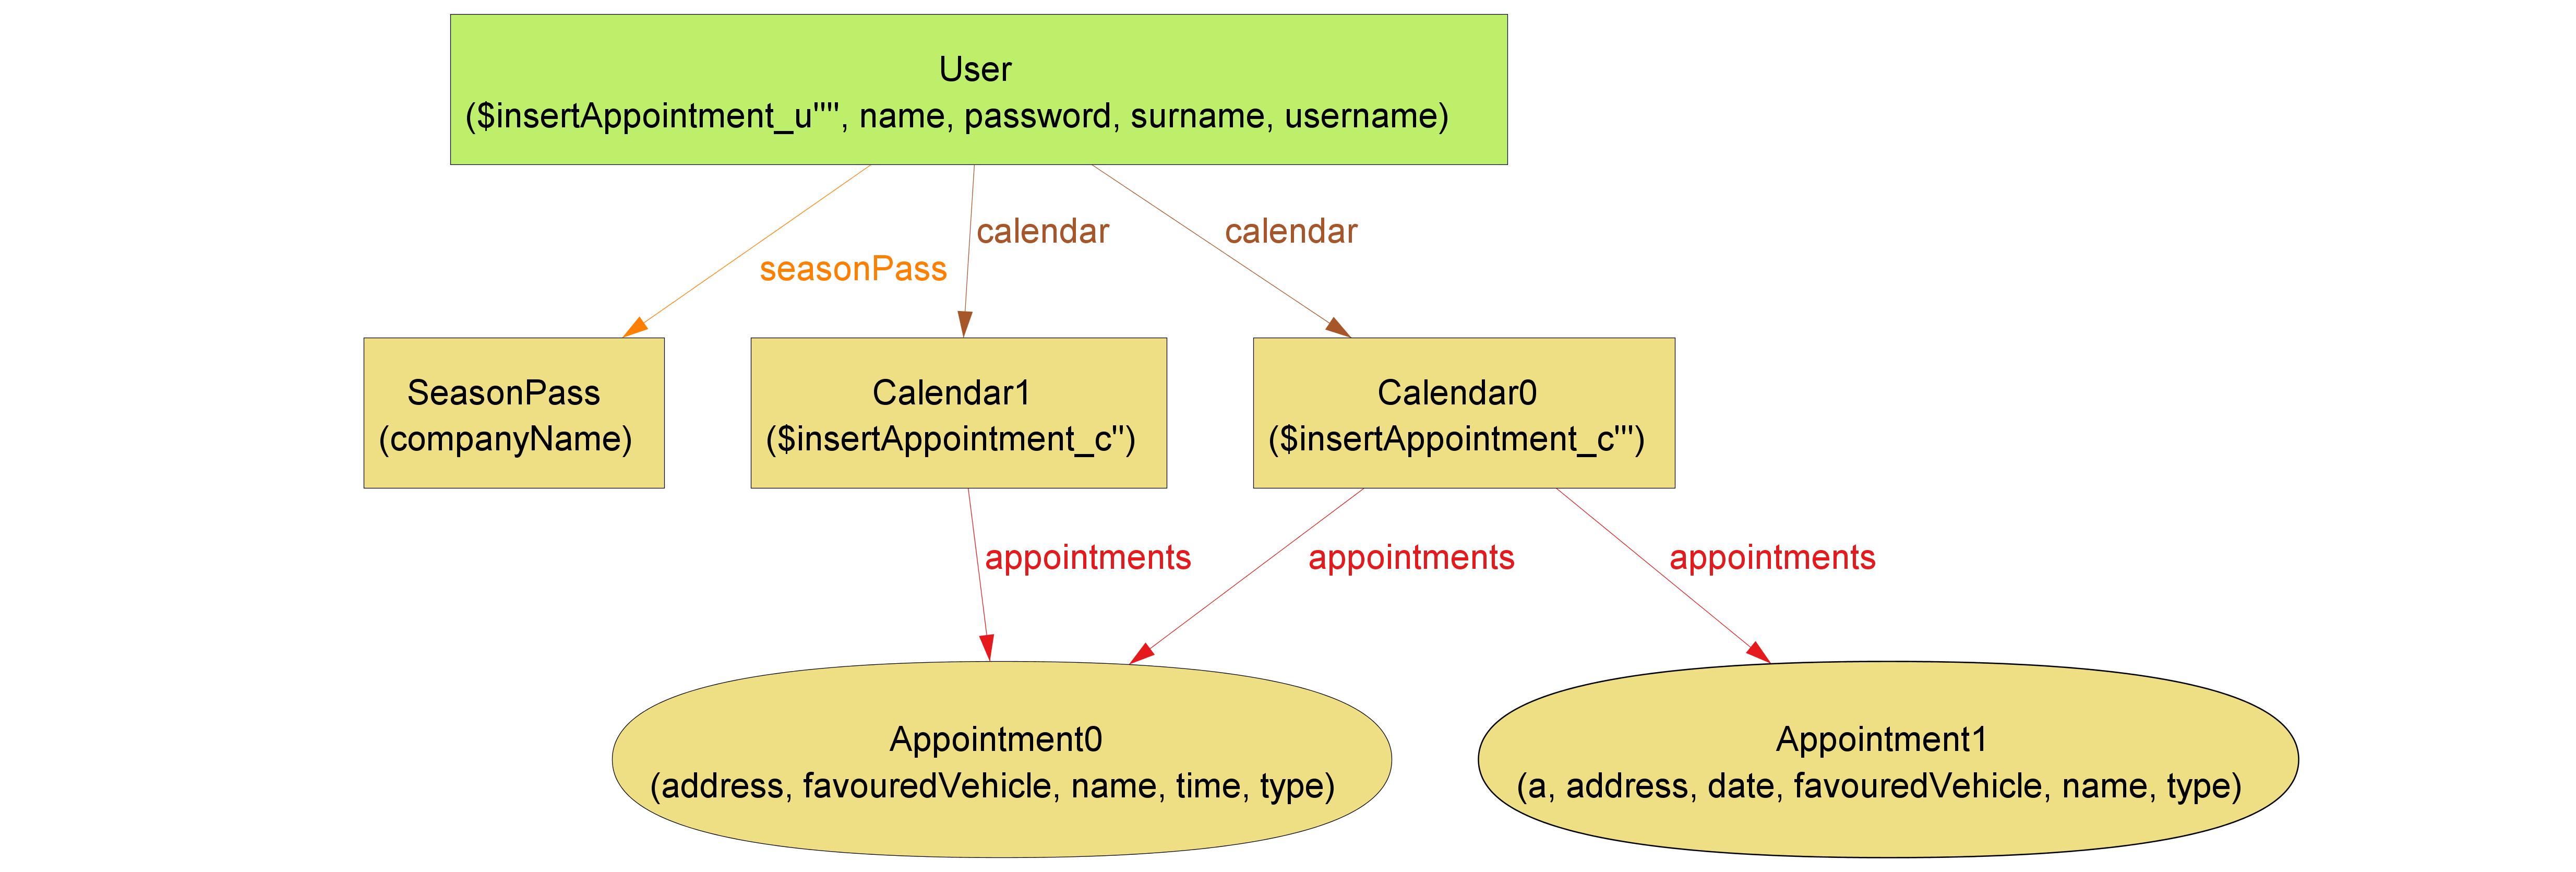
\includegraphics[height = 0.7\textheight, width= 25cm, center]{alloy/generatedWorld/insertAppointment}

\end{landscape}
	
	
